For the final Milestone, each group member was required to individually implement different Barrelfish subsystems and then jointly integrate them at the end. This chapter delves into \textit{capabilities} and was completed by \textbf{Arya}.

\subsection{Introduction}
To fully leverage the power of Barrelfish's capability system, some additional capability operations needed to be implemented. 
\\\\
First, adding the ability to share capabilities across cores allows for more powerful communication between them. Proper tracking of shared capabilities increases the safety of services that hand out capabilities to the other core, like the memory server.
\\\\
Additionally, \texttt{delete}, \texttt{revoke}, and \texttt{retype} operations are always sent first to the kernel through a system call, but there are some situations where the kernel is not properly able to handle the request, and instead leaves the responsibility to the monitor. Some of these situations are as follows:
\\
\begin{itemize}
    \item \textbf{Deleting a CNode or Dispatcher capability}: These types of capabilities contain additional capability slots within them. The internal capabilities need to be deleted as well, but this will take multiple steps, and in keeping with the microkernel architecture, the kernal should not perform a long-running operation like this. 
    \item \textbf{Revoking a capability}: Similarly, the kernel should not revoke a capability, because doing so could involve many delete steps (eg. deleting a number of descendants).
    \item \textbf{Deleting the last copy of a shared capability}: If a capability is shared between cores, the monitor needs to negotiate the deletion.
    \item \textbf{Revoking a shared capability}: Similarly, when revoking a shared capability, the monitor needs to ensure that the capability is revoked over the entire system.
    \item \textbf{Retyping a shared capability}: To maintain capability invariants, the monitor needs to check with the remote core as well as the local one to ensure a retype operation is legal.
    \item \textbf{Deleting the last copy of a mem-backed capability}: When the last copy of a capability that refers to physical memory is deleted, the monitor is invoked so that it can notify the memory manager and thus free the resource for future allocation.
\end{itemize}
\subsection{Handling Operations in the Monitor}
\noindent
When system capability operations fail with the error code \texttt{SYS\_ERR\_RETRY\_THROUGH\_MONITOR}, the child process sends an LMP message to its local monitor containing its root CNode, and the address of the relevant capability. The monitor is able to complete the operation on the capability, even though it is from a different CSpace, by referring to the child dispatcher's root CNode.
\\\\
Some operations are sent to the monitor because they would take too long for a single syscall. This occurs when deleting a CNode or Dispatcher capability, or when revoking a capability. The monitor first marks all relevant capabilities for deletion, which creates a queue of delete steps. Each delete step can be completed as a single syscall, and the monitor iterates through the delete steps until all are completed. Once complete, it sends an LMP acknowledgement to the child to indicate that the process has completed. \\
This way, each syscall completes in a bounded time, which is one of the invariants necessary for a stateless kernel.

\subsection{Distributed Capabilities}

Some precautions need to be taken for distributed capabilities to ensure a safe system state. Every capability has a specified owning core, every copy of the same capabilities must have the same specified owner, and the owning core must always have a copy of all capabilities it owns. The first step of ensuring these invariants happens when a capability is shared between cores.
\\\\
To share a capability with another core, a process sends a request to its local monitor (if it is not already the monitor). While the monitor can identify and perform operations on capabilities in a child process' CSpace by referring to the child's root CNode, it cannot do this for capabilities on another core. For that reason, whenever a capability is going to be transferred cross-core, the monitor generates a unique key for it, and stores the key and capability in a hash table. It sends the capability information to the other core along with the generated key, and the other core's monitor creates a local copy of the capability and stores it with the shared key in its own hashtable.
\\\\
The monitors both set the same owner of the capability as specified in the transfer message, and set each capability's remote relations metadata to indicate that they have a remote copy. As a result, the kernel will pass certain operations (like deleting the last copy on this core) up to the monitor to handle.
\\\\
For any cross-core operations involving shared capabilities, the cores can communicate efficiently using the shared key of the capability (see Figure \ref{figure:m7_shared_key}).

\begin{figure}[ht]
    \centering
    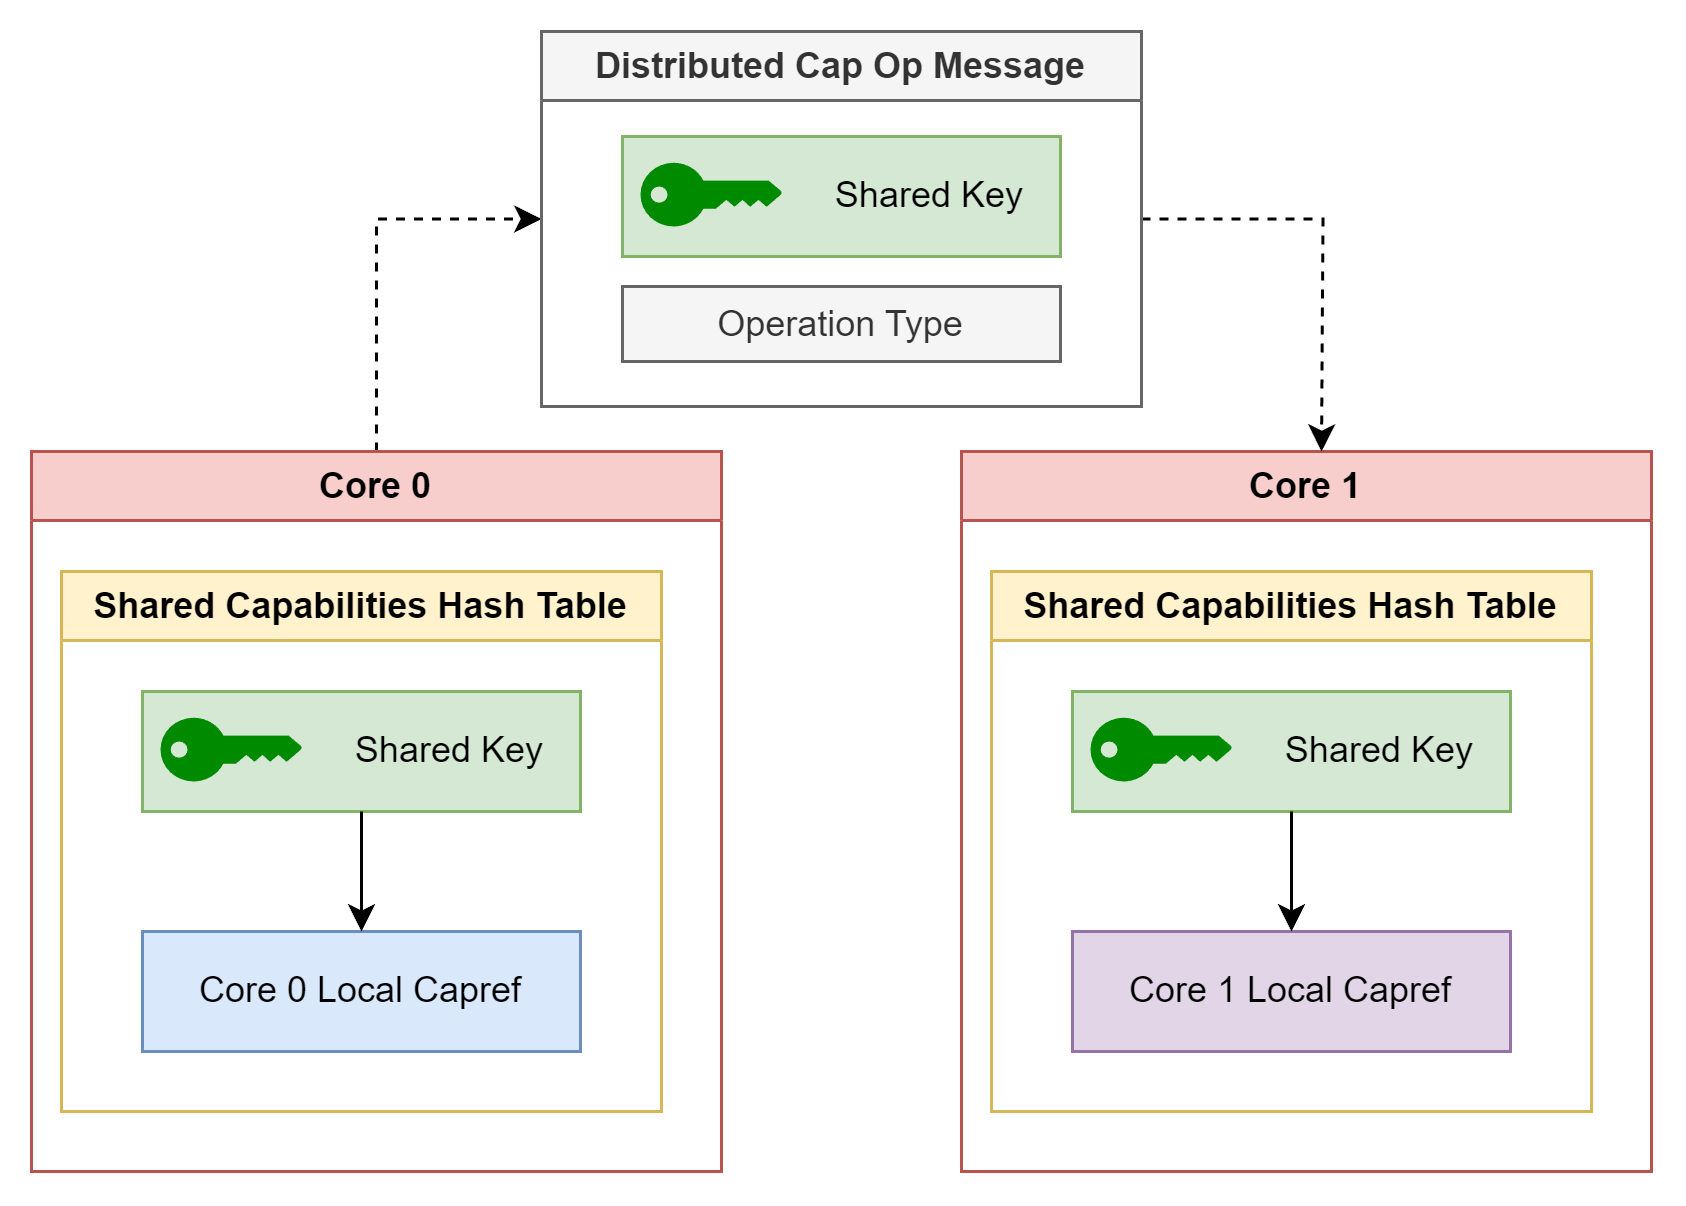
\includegraphics[width=0.8\columnwidth]{images/capability_ops.png}
    \caption{Cross-core capability operations using a shared key}
    \label{figure:m7_shared_key}
\end{figure}

\subsection{Coordinating Distributed Operations}

\textbf{Deletion}: 
When the last local copy of a shared capability is deleted, the local monitor is notified. There are three potential cases: \\
\begin{enumerate}
    \item If the capability is owned by the local core and ownership is transferable, the monitor sends a \texttt{TRANSFER\_OWNERSHIP} message to the remote core, then deletes its local copy. Once the remote core acknowledges the transfer of ownership, the deletion is complete.
    \item If the capability is owned by the local core but the capability type cannot have its ownership transferred (eg. a dispatcher capability), then the remote core is sent a \texttt{DELETE\_ALL} message notifying it to delete its local capabilities. When the remote core acknowledges completion, the deletion is complete.
    \item If the capability is not owned by this core, the monitor sends a \texttt{NOTIFY\_DELETED} message to the other core. This step is not strictly necessary, but it allows the other core to delete any metadata for the capability that is no longer needed (eg. in the shared capability hashtable), and to update the remote relations of the capability.
\end{enumerate}
\\
\textbf{Revocation}: Revocation of a capability should ensure that no copies or descendants exist in the entire system, not only in the local core. When a shared capability is revoked, regardless of which core owns the capability, the other core needs to be notified to delete any copies and descendants. The monitor marks its local copies and descendants for deletion, then sends \texttt{DELETE\_ALL} message to the other core. The other core marks and deletes its own copies and descendants, then replies with a \texttt{DELETE\_SWEEP} message, triggering the original core to complete its local delete steps and complete the operation.
\\\\
\textbf{Retyping}: Retype operations are illegal in certain situations, such as when another descendant already exists. For consistency, this invariant must be maintained system-wide, not only on the local core. When a retype operation is invoked on a shared capability, the operation is sent to the monitor. The monitor sends a \texttt{CAN\_RETYPE} message to the other core. The other core checks for local descendants of the shared capability, and responds YES or NO. If YES, the local monitor can successfully perform the retype operation. If NO, the operation fails because it is not a legal retype.

\subsection{Shared Capabilities and Concurrency}

The shared capability operations present some issues if used concurrently. To help mitigate this, the monitor is able to "lock" a capability to indicate that no other concurrent operation should be performed on it. For example the monitor locks a capability when trying to perform a retype on it, and also locks the capability when the remote core requests to check if the capability can be retyped. This prevents the monitor from providing inconsistent answers (eg. it tells the other core that it can retype the shared capability, while simultaneously retyping the capability locally).
However, it is a difficult task to ensure that no conflicting operations ever occur. If designing an OS for deployment, each possible concurrent operation would have to be considered. Barrelfish implements a "Two-Phase-Commit" protocol to better guard against inconsistencies due to concurrency, but this would have been too complicated to implement in the given time.

\subsection{Memory Server Integration}
The memory server was first introduced in M4, but it was revisited during this milestone because it was modified to use the safe capability sharing operations. This modification also unearthed some existing issues with the memory server implementation.
\\\\
\textbf{Memory Distribution}:
We chose to implement core 0 as the main memory server, so that most memory would be consolidated in one place, and core 1 is able to request more memory as necessary. An advantage of this approach is that memory only needs to be requested in one direction, preventing potential complications of both cores requesting memory from eachother. A disadvantage is that the overhead of memory operations is increased when core 1 needs a lot of memory. If the OS were to be used for a particular workload where the programmer was aware of where memory would be needed most, they might choose to implement this differently to optimize memory access.
\\\\
The monitor on core 1 can request RAM capabilities from core 0, and child processes on either core and request RAM from their local monitor. When child processes request memory from core 1's monitor, it forwards the request to core 0.
\\\\
\textbf{Sharing Memory with Distributed Capabilities}:
A benefit of the distributed capabilities system is it allows for a better memory server implementation. Previously, when requesting RAM from the other core, the unsafe \texttt{ram\_forge} operation was necessary to create a RAM cap on the receiving core. Now, the capability is sent safely, and the ownership is transferred to the receiving core. This choice was made so that the memory server does not need to keep a copy of the RAM, and the child process does not need to invoke the monitor constantly when performing local operations on the received RAM. Only when the last copy of the memory is deleted on the receiving core, and operation is sent to the monitor, does the monitor sends a RAM capability back to the memory server to free. In fact, any cap that is backed by physical memory will trigger the memory to be freed automatically when the last copy of the capability is deleted. This is a powerful effect of the capability system, and ensures that memory leaks do not occur as long as capabilities are cleaned up correctly.
\\\\
\textbf{Coordinating Remote RAM Requests}:
Coordinating processes to correctly request remote RAM proved to be more difficult than expected. The crux of the issue was that sending and receiving an RPC call requires RAM itself, so a process/core cannot wait until it is out of memory to request more. This issue is reminiscent of the memory threshold for Memory Manager in M1. However, there is more difficulty here because child processes do not have a memory manager; they begin with a capability to some initial starting memory, then any additional memory needs to be requested from the memory server. There is no way to "refill" and manage the starting memory. For this, we would need to initialize a memory manager in every dispatcher, and refill it with memory from a monitor.
\\\\
To prevent infinite loops, we implemented a flag that prevents a process from requesting remote memory while it is in the process of requesting remote memory, or while servicing a page fault. This imposes severe limitations on the memory sharing system. Each dispatcher starts with a fixed amount of "starting memory", and it requests remote RAM to serve allocation requests whenever possible, but falls back on the starting memory in the indicated situations. This means that a dispatcher will eventually run out of memory, even when there may be plenty of additional memory in the monitor.
\\\\
\textbf{Alternate Sharing Designs}: 
There are several other ways that RAM capabilities might be shared between cores.
\begin{itemize}
    \item Initially, we considered the possibility that the memory server's core maintains ownership of sent capabilities. However, this would cause additional overhead in the form of metadata (shared capabilities in the monitors' hash tables), and more capability operations on the receiving core would trigger the monitor. The idea was abandoned for this reason.
    \item Another option, as mentioned earlier, would be for each dispatcher to have its own memory manager. When the memory available falls below a certain threshold, it would request a large chunk of memory to add. This has the advantage of reducing the number of RPC calls in the system and preventing dispatchers from prematurely running out of memory. A disadvantage is that this could cause greater memory fragmentation, since dispatchers would be holding large chunks of memory which may not be freed for a long period of time (or until the process exits). This design seems promising, but it would introduce additional complexity, and the memory manager was not designed to be used outside of the monitor. We chose not to take the risk of doing so now.
\end{itemize}
\subsection{Challenges}
A particular challenge with this milestone was "filling in the blanks" of the monitor with respect to the underlying kernel code. In some cases it became apparent that the kernel code for capability operations was made for a different monitor design. In some cases I modified the checks in order to pass operations up to the monitor that previously would not have been, because my design required it. For example, I modified the kernel code to pass retype operations up to the monitor for any capability with remote copies, not only remote descendants. This was necessary since, in my implementation, a monitor will not necessarily be notified when the other core does a local retype, so it will not know that the capability has remote descendants. My solution was to always pass the retype operation for shared capabilities up to the monitor so that the monitor can query the other core for descendants.

\subsection{Conclusion}
The completed deliverables are all demonstrated in the \texttt{capabilities\_m7} binary, which expects to be run on core 1 so that it gets RAM capabilities from the remote core. The implemented functionalities are:
\begin{itemize}
    \item The monitor can receive and process capability operations.
    \item \texttt{cap\_revoke} and \texttt{cap\_delete} work on a single core for any capability.
    \item Can send capabilities cross core over UMP with the right remote relations (I did not implement spawn with caps cross core, but used a \texttt{send\_cap\_remote} RPC call to test the functionality).
    \item Handle \texttt{cap\_delete}, \texttt{cap\_revoke}, \texttt{cap\_retype} for any capability including ownership transfer and remote relations.
    \item Use the capability transfer mechanism cross core in the memory allocation system.
    \item Return no-longer used memory back to the memory server.
\end{itemize}
